% Created by tikzDevice version 0.12.6 on 2026-08-14 08:42:30
% !TEX encoding = UTF-8 Unicode
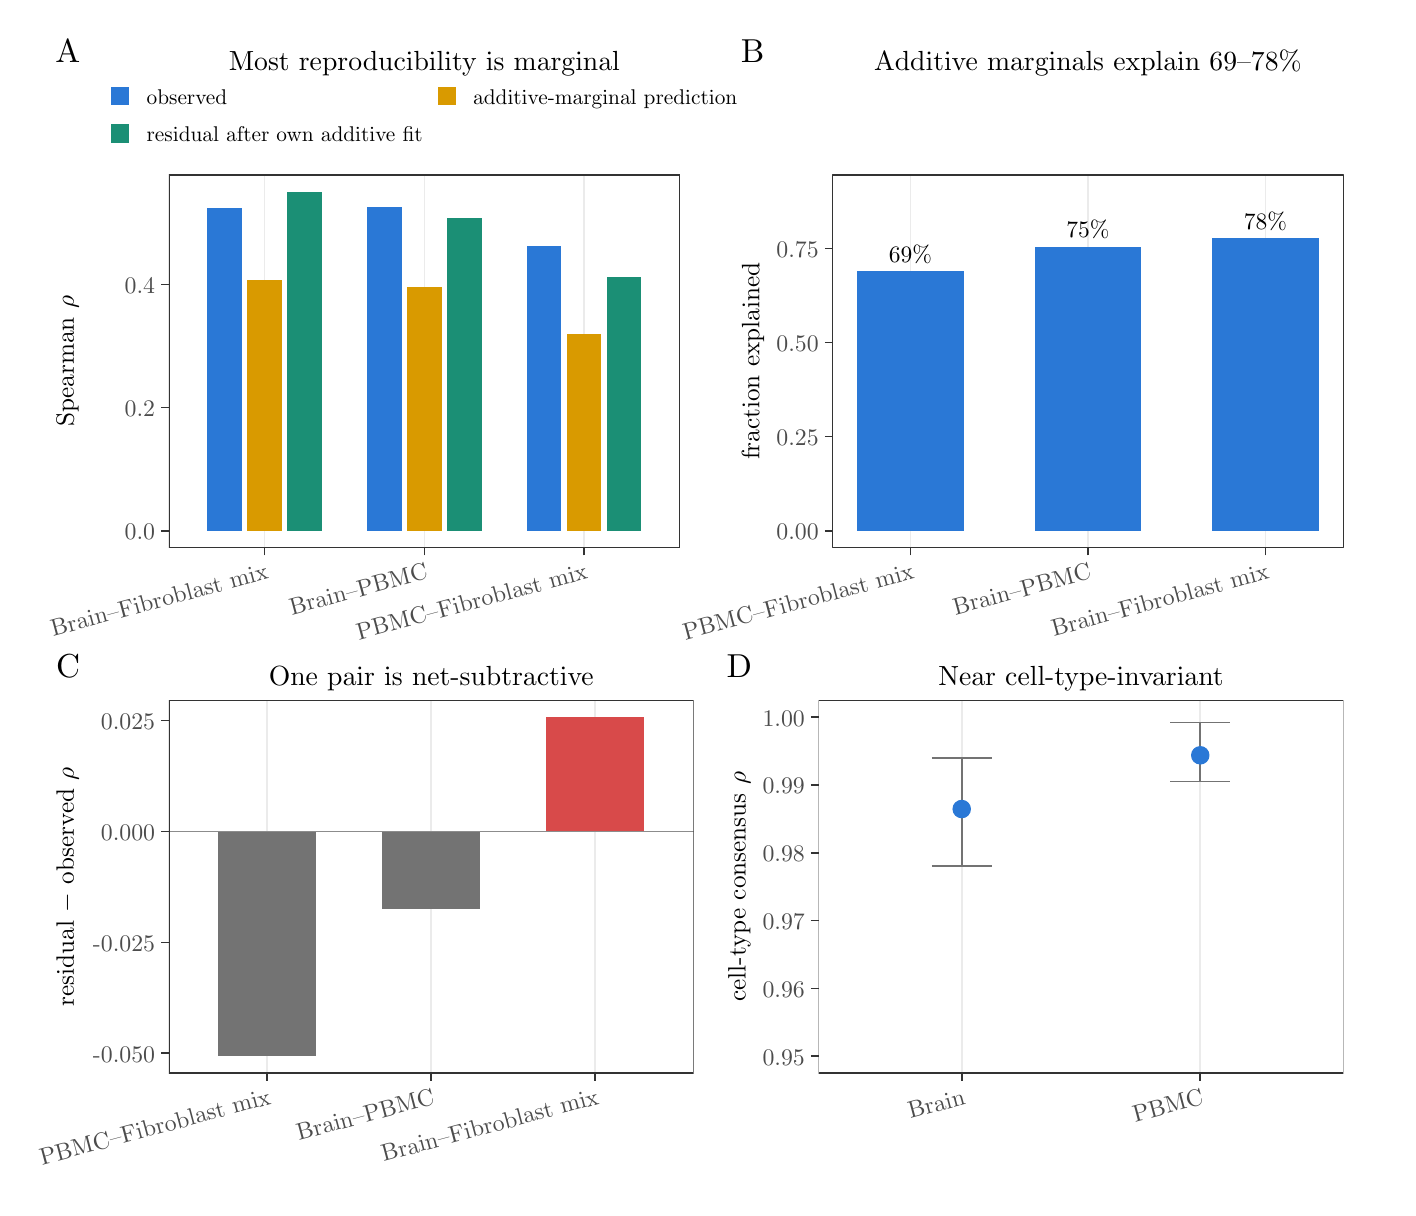
\begin{tikzpicture}[x=1pt,y=1pt]
\definecolor{fillColor}{RGB}{255,255,255}
\path[use as bounding box,fill=fillColor,fill opacity=0.00] (0,0) rectangle (491.44,419.17);
\begin{scope}
\path[clip] (  0.00,  0.00) rectangle (491.44,419.17);
\definecolor{drawColor}{RGB}{255,255,255}
\definecolor{fillColor}{RGB}{255,255,255}

\path[draw=drawColor,line width= 0.6pt,line join=round,line cap=round,fill=fillColor] (  0.00,  0.00) rectangle (491.44,419.17);
\end{scope}
\begin{scope}
\path[clip] (  4.00,192.87) rectangle (249.66,415.17);
\definecolor{drawColor}{RGB}{255,255,255}
\definecolor{fillColor}{RGB}{255,255,255}

\path[draw=drawColor,line width= 0.6pt,line join=round,line cap=round,fill=fillColor] (  4.00,192.87) rectangle (249.66,415.17);
\end{scope}
\begin{scope}
\path[clip] (249.66,192.87) rectangle (485.44,415.17);
\definecolor{drawColor}{RGB}{255,255,255}
\definecolor{fillColor}{RGB}{255,255,255}

\path[draw=drawColor,line width= 0.6pt,line join=round,line cap=round,fill=fillColor] (249.66,192.87) rectangle (485.44,415.17);
\end{scope}
\begin{scope}
\path[clip] ( 51.01,231.27) rectangle (235.66,365.96);
\definecolor{fillColor}{RGB}{255,255,255}

\path[fill=fillColor] ( 51.01,231.27) rectangle (235.66,365.96);
\definecolor{drawColor}{gray}{0.92}

\path[draw=drawColor,line width= 0.6pt,line join=round] ( 85.63,231.27) --
	( 85.63,365.96);

\path[draw=drawColor,line width= 0.6pt,line join=round] (143.33,231.27) --
	(143.33,365.96);

\path[draw=drawColor,line width= 0.6pt,line join=round] (201.04,231.27) --
	(201.04,365.96);
\definecolor{fillColor}{RGB}{42,120,214}

\path[fill=fillColor] (122.66,237.39) rectangle (135.16,354.19);

\path[fill=fillColor] ( 64.96,237.39) rectangle ( 77.46,354.11);

\path[fill=fillColor] (180.36,237.39) rectangle (192.86,340.28);
\definecolor{fillColor}{RGB}{217,154,0}

\path[fill=fillColor] (137.08,237.39) rectangle (149.58,325.50);

\path[fill=fillColor] ( 79.38,237.39) rectangle ( 91.88,328.10);

\path[fill=fillColor] (194.78,237.39) rectangle (207.29,308.33);
\definecolor{fillColor}{RGB}{27,143,117}

\path[fill=fillColor] (151.51,237.39) rectangle (164.01,350.30);

\path[fill=fillColor] ( 93.81,237.39) rectangle (106.31,359.84);

\path[fill=fillColor] (209.21,237.39) rectangle (221.71,329.01);
\definecolor{drawColor}{gray}{0.20}

\path[draw=drawColor,line width= 0.6pt,line join=round,line cap=round] ( 51.01,231.27) rectangle (235.66,365.96);
\end{scope}
\begin{scope}
\path[clip] (  0.00,  0.00) rectangle (491.44,419.17);
\definecolor{drawColor}{gray}{0.30}

\node[text=drawColor,anchor=base east,inner sep=0pt, outer sep=0pt, scale=  0.86] at ( 46.06,234.19) {0.0};

\node[text=drawColor,anchor=base east,inner sep=0pt, outer sep=0pt, scale=  0.86] at ( 46.06,278.70) {0.2};

\node[text=drawColor,anchor=base east,inner sep=0pt, outer sep=0pt, scale=  0.86] at ( 46.06,323.21) {0.4};
\end{scope}
\begin{scope}
\path[clip] (  0.00,  0.00) rectangle (491.44,419.17);
\definecolor{drawColor}{gray}{0.20}

\path[draw=drawColor,line width= 0.6pt,line join=round] ( 48.26,237.39) --
	( 51.01,237.39);

\path[draw=drawColor,line width= 0.6pt,line join=round] ( 48.26,281.90) --
	( 51.01,281.90);

\path[draw=drawColor,line width= 0.6pt,line join=round] ( 48.26,326.41) --
	( 51.01,326.41);
\end{scope}
\begin{scope}
\path[clip] (  0.00,  0.00) rectangle (491.44,419.17);
\definecolor{drawColor}{gray}{0.20}

\path[draw=drawColor,line width= 0.6pt,line join=round] ( 85.63,228.52) --
	( 85.63,231.27);

\path[draw=drawColor,line width= 0.6pt,line join=round] (143.33,228.52) --
	(143.33,231.27);

\path[draw=drawColor,line width= 0.6pt,line join=round] (201.04,228.52) --
	(201.04,231.27);
\end{scope}
\begin{scope}
\path[clip] (  0.00,  0.00) rectangle (491.44,419.17);
\definecolor{drawColor}{gray}{0.30}

\node[text=drawColor,rotate= 15.00,anchor=base east,inner sep=0pt, outer sep=0pt, scale=  0.86] at ( 87.29,220.14) {Brain--Fibroblast mix};

\node[text=drawColor,rotate= 15.00,anchor=base east,inner sep=0pt, outer sep=0pt, scale=  0.86] at (144.99,220.14) {Brain--PBMC};

\node[text=drawColor,rotate= 15.00,anchor=base east,inner sep=0pt, outer sep=0pt, scale=  0.86] at (202.69,220.14) {PBMC--Fibroblast mix};
\end{scope}
\begin{scope}
\path[clip] (  0.00,  0.00) rectangle (491.44,419.17);
\definecolor{drawColor}{RGB}{0,0,0}

\node[text=drawColor,rotate= 90.00,anchor=base,inner sep=0pt, outer sep=0pt, scale=  0.91] at ( 16.73,298.61) {Spearman $\rho$};
\end{scope}
\begin{scope}
\path[clip] (  0.00,  0.00) rectangle (491.44,419.17);
\definecolor{fillColor}{RGB}{255,255,255}

\path[fill=fillColor] ( 29.51,376.96) rectangle (257.15,398.39);
\end{scope}
\begin{scope}
\path[clip] (  0.00,  0.00) rectangle (491.44,419.17);
\definecolor{fillColor}{RGB}{255,255,255}

\path[fill=fillColor] ( 29.51,390.43) rectangle ( 37.48,398.39);
\definecolor{fillColor}{RGB}{42,120,214}

\path[fill=fillColor] ( 30.23,391.14) rectangle ( 36.77,397.68);
\end{scope}
\begin{scope}
\path[clip] (  0.00,  0.00) rectangle (491.44,419.17);
\definecolor{fillColor}{RGB}{255,255,255}

\path[fill=fillColor] (147.53,390.43) rectangle (155.49,398.39);
\definecolor{fillColor}{RGB}{217,154,0}

\path[fill=fillColor] (148.24,391.14) rectangle (154.78,397.68);
\end{scope}
\begin{scope}
\path[clip] (  0.00,  0.00) rectangle (491.44,419.17);
\definecolor{fillColor}{RGB}{255,255,255}

\path[fill=fillColor] ( 29.51,376.96) rectangle ( 37.48,384.93);
\definecolor{fillColor}{RGB}{27,143,117}

\path[fill=fillColor] ( 30.23,377.67) rectangle ( 36.77,384.22);
\end{scope}
\begin{scope}
\path[clip] (  0.00,  0.00) rectangle (491.44,419.17);
\definecolor{drawColor}{RGB}{0,0,0}

\node[text=drawColor,anchor=base west,inner sep=0pt, outer sep=0pt, scale=  0.77] at ( 42.98,391.55) {observed};
\end{scope}
\begin{scope}
\path[clip] (  0.00,  0.00) rectangle (491.44,419.17);
\definecolor{drawColor}{RGB}{0,0,0}

\node[text=drawColor,anchor=base west,inner sep=0pt, outer sep=0pt, scale=  0.77] at (160.99,391.55) {additive-marginal prediction};
\end{scope}
\begin{scope}
\path[clip] (  0.00,  0.00) rectangle (491.44,419.17);
\definecolor{drawColor}{RGB}{0,0,0}

\node[text=drawColor,anchor=base west,inner sep=0pt, outer sep=0pt, scale=  0.77] at ( 42.98,378.08) {residual after own additive fit};
\end{scope}
\begin{scope}
\path[clip] (  0.00,  0.00) rectangle (491.44,419.17);
\definecolor{drawColor}{RGB}{0,0,0}

\node[text=drawColor,anchor=base,inner sep=0pt, outer sep=0pt, scale=  1.00] at (143.33,403.76) {Most reproducibility is marginal};
\end{scope}
\begin{scope}
\path[clip] (  0.00,  0.00) rectangle (491.44,419.17);
\definecolor{drawColor}{RGB}{0,0,0}

\node[text=drawColor,anchor=base,inner sep=0pt, outer sep=0pt, scale=  1.20] at ( 14.51,406.72) {A};
\end{scope}
\begin{scope}
\path[clip] (  0.00,  0.00) rectangle (491.44,419.17);
\definecolor{fillColor}{RGB}{255,255,255}

\path[fill=fillColor] (290.79,231.27) rectangle (475.44,365.96);
\definecolor{drawColor}{gray}{0.92}

\path[draw=drawColor,line width= 0.6pt,line join=round] (319.00,231.27) --
	(319.00,365.96);

\path[draw=drawColor,line width= 0.6pt,line join=round] (383.11,231.27) --
	(383.11,365.96);

\path[draw=drawColor,line width= 0.6pt,line join=round] (447.23,231.27) --
	(447.23,365.96);
\definecolor{fillColor}{RGB}{42,120,214}

\path[fill=fillColor] (363.88,237.39) rectangle (402.35,340.01);

\path[fill=fillColor] (427.99,237.39) rectangle (466.46,343.12);

\path[fill=fillColor] (299.77,237.39) rectangle (338.23,331.20);
\definecolor{drawColor}{RGB}{0,0,0}

\node[text=drawColor,anchor=base,inner sep=0pt, outer sep=0pt, scale=  0.85] at (383.11,343.17) {75\%};

\node[text=drawColor,anchor=base,inner sep=0pt, outer sep=0pt, scale=  0.85] at (447.23,346.28) {78\%};

\node[text=drawColor,anchor=base,inner sep=0pt, outer sep=0pt, scale=  0.85] at (319.00,334.36) {69\%};
\definecolor{drawColor}{gray}{0.20}

\path[draw=drawColor,line width= 0.6pt,line join=round,line cap=round] (290.79,231.27) rectangle (475.44,365.96);
\end{scope}
\begin{scope}
\path[clip] (  0.00,  0.00) rectangle (491.44,419.17);
\definecolor{drawColor}{gray}{0.30}

\node[text=drawColor,anchor=base east,inner sep=0pt, outer sep=0pt, scale=  0.86] at (285.84,234.19) {0.00};

\node[text=drawColor,anchor=base east,inner sep=0pt, outer sep=0pt, scale=  0.86] at (285.84,268.21) {0.25};

\node[text=drawColor,anchor=base east,inner sep=0pt, outer sep=0pt, scale=  0.86] at (285.84,302.22) {0.50};

\node[text=drawColor,anchor=base east,inner sep=0pt, outer sep=0pt, scale=  0.86] at (285.84,336.23) {0.75};
\end{scope}
\begin{scope}
\path[clip] (  0.00,  0.00) rectangle (491.44,419.17);
\definecolor{drawColor}{gray}{0.20}

\path[draw=drawColor,line width= 0.6pt,line join=round] (288.04,237.39) --
	(290.79,237.39);

\path[draw=drawColor,line width= 0.6pt,line join=round] (288.04,271.40) --
	(290.79,271.40);

\path[draw=drawColor,line width= 0.6pt,line join=round] (288.04,305.42) --
	(290.79,305.42);

\path[draw=drawColor,line width= 0.6pt,line join=round] (288.04,339.43) --
	(290.79,339.43);
\end{scope}
\begin{scope}
\path[clip] (  0.00,  0.00) rectangle (491.44,419.17);
\definecolor{drawColor}{gray}{0.20}

\path[draw=drawColor,line width= 0.6pt,line join=round] (319.00,228.52) --
	(319.00,231.27);

\path[draw=drawColor,line width= 0.6pt,line join=round] (383.11,228.52) --
	(383.11,231.27);

\path[draw=drawColor,line width= 0.6pt,line join=round] (447.23,228.52) --
	(447.23,231.27);
\end{scope}
\begin{scope}
\path[clip] (  0.00,  0.00) rectangle (491.44,419.17);
\definecolor{drawColor}{gray}{0.30}

\node[text=drawColor,rotate= 15.00,anchor=base east,inner sep=0pt, outer sep=0pt, scale=  0.86] at (320.65,220.14) {PBMC--Fibroblast mix};

\node[text=drawColor,rotate= 15.00,anchor=base east,inner sep=0pt, outer sep=0pt, scale=  0.86] at (384.77,220.14) {Brain--PBMC};

\node[text=drawColor,rotate= 15.00,anchor=base east,inner sep=0pt, outer sep=0pt, scale=  0.86] at (448.88,220.14) {Brain--Fibroblast mix};
\end{scope}
\begin{scope}
\path[clip] (  0.00,  0.00) rectangle (491.44,419.17);
\definecolor{drawColor}{RGB}{0,0,0}

\node[text=drawColor,rotate= 90.00,anchor=base,inner sep=0pt, outer sep=0pt, scale=  0.91] at (264.39,298.61) {fraction explained};
\end{scope}
\begin{scope}
\path[clip] (  0.00,  0.00) rectangle (491.44,419.17);
\definecolor{drawColor}{RGB}{0,0,0}

\node[text=drawColor,anchor=base,inner sep=0pt, outer sep=0pt, scale=  1.00] at (383.11,403.76) {Additive marginals explain 69--78\%};
\end{scope}
\begin{scope}
\path[clip] (  0.00,  0.00) rectangle (491.44,419.17);
\definecolor{drawColor}{RGB}{0,0,0}

\node[text=drawColor,anchor=base,inner sep=0pt, outer sep=0pt, scale=  1.20] at (262.01,406.72) {B};
\end{scope}
\begin{scope}
\path[clip] (  4.00,  3.00) rectangle (246.66,192.87);
\definecolor{drawColor}{RGB}{255,255,255}
\definecolor{fillColor}{RGB}{255,255,255}

\path[draw=drawColor,line width= 0.6pt,line join=round,line cap=round,fill=fillColor] (  4.00,  3.00) rectangle (246.66,192.87);
\end{scope}
\begin{scope}
\path[clip] (246.66,  3.00) rectangle (485.44,192.87);
\definecolor{drawColor}{RGB}{255,255,255}
\definecolor{fillColor}{RGB}{255,255,255}

\path[draw=drawColor,line width= 0.6pt,line join=round,line cap=round,fill=fillColor] (246.66,  3.00) rectangle (485.44,192.87);
\end{scope}
\begin{scope}
\path[clip] ( 51.01, 41.40) rectangle (240.66,176.09);
\definecolor{fillColor}{RGB}{255,255,255}

\path[fill=fillColor] ( 51.01, 41.40) rectangle (240.66,176.09);
\definecolor{drawColor}{gray}{0.92}

\path[draw=drawColor,line width= 0.6pt,line join=round] ( 86.57, 41.40) --
	( 86.57,176.09);

\path[draw=drawColor,line width= 0.6pt,line join=round] (145.83, 41.40) --
	(145.83,176.09);

\path[draw=drawColor,line width= 0.6pt,line join=round] (205.10, 41.40) --
	(205.10,176.09);
\definecolor{fillColor}{gray}{0.45}

\path[fill=fillColor] (128.05,100.64) rectangle (163.61,128.73);
\definecolor{fillColor}{RGB}{216,74,74}

\path[fill=fillColor] (187.32,128.73) rectangle (222.88,169.97);
\definecolor{fillColor}{gray}{0.45}

\path[fill=fillColor] ( 68.79, 47.52) rectangle (104.35,128.73);
\definecolor{drawColor}{gray}{0.55}

\path[draw=drawColor,line width= 0.6pt,line join=round] ( 51.01,128.73) -- (240.66,128.73);
\definecolor{drawColor}{gray}{0.20}

\path[draw=drawColor,line width= 0.6pt,line join=round,line cap=round] ( 51.01, 41.40) rectangle (240.66,176.09);
\end{scope}
\begin{scope}
\path[clip] (  0.00,  0.00) rectangle (491.44,419.17);
\definecolor{drawColor}{gray}{0.30}

\node[text=drawColor,anchor=base east,inner sep=0pt, outer sep=0pt, scale=  0.86] at ( 46.06, 45.36) {-0.050};

\node[text=drawColor,anchor=base east,inner sep=0pt, outer sep=0pt, scale=  0.86] at ( 46.06, 85.45) {-0.025};

\node[text=drawColor,anchor=base east,inner sep=0pt, outer sep=0pt, scale=  0.86] at ( 46.06,125.54) {0.000};

\node[text=drawColor,anchor=base east,inner sep=0pt, outer sep=0pt, scale=  0.86] at ( 46.06,165.62) {0.025};
\end{scope}
\begin{scope}
\path[clip] (  0.00,  0.00) rectangle (491.44,419.17);
\definecolor{drawColor}{gray}{0.20}

\path[draw=drawColor,line width= 0.6pt,line join=round] ( 48.26, 48.55) --
	( 51.01, 48.55);

\path[draw=drawColor,line width= 0.6pt,line join=round] ( 48.26, 88.64) --
	( 51.01, 88.64);

\path[draw=drawColor,line width= 0.6pt,line join=round] ( 48.26,128.73) --
	( 51.01,128.73);

\path[draw=drawColor,line width= 0.6pt,line join=round] ( 48.26,168.82) --
	( 51.01,168.82);
\end{scope}
\begin{scope}
\path[clip] (  0.00,  0.00) rectangle (491.44,419.17);
\definecolor{drawColor}{gray}{0.20}

\path[draw=drawColor,line width= 0.6pt,line join=round] ( 86.57, 38.65) --
	( 86.57, 41.40);

\path[draw=drawColor,line width= 0.6pt,line join=round] (145.83, 38.65) --
	(145.83, 41.40);

\path[draw=drawColor,line width= 0.6pt,line join=round] (205.10, 38.65) --
	(205.10, 41.40);
\end{scope}
\begin{scope}
\path[clip] (  0.00,  0.00) rectangle (491.44,419.17);
\definecolor{drawColor}{gray}{0.30}

\node[text=drawColor,rotate= 15.00,anchor=base east,inner sep=0pt, outer sep=0pt, scale=  0.86] at ( 88.22, 30.28) {PBMC--Fibroblast mix};

\node[text=drawColor,rotate= 15.00,anchor=base east,inner sep=0pt, outer sep=0pt, scale=  0.86] at (147.49, 30.28) {Brain--PBMC};

\node[text=drawColor,rotate= 15.00,anchor=base east,inner sep=0pt, outer sep=0pt, scale=  0.86] at (206.75, 30.28) {Brain--Fibroblast mix};
\end{scope}
\begin{scope}
\path[clip] (  0.00,  0.00) rectangle (491.44,419.17);
\definecolor{drawColor}{RGB}{0,0,0}

\node[text=drawColor,rotate= 90.00,anchor=base,inner sep=0pt, outer sep=0pt, scale=  0.91] at ( 16.73,108.75) {residual $-$ observed $\rho$};
\end{scope}
\begin{scope}
\path[clip] (  0.00,  0.00) rectangle (491.44,419.17);
\definecolor{drawColor}{RGB}{0,0,0}

\node[text=drawColor,anchor=base,inner sep=0pt, outer sep=0pt, scale=  1.00] at (145.83,181.46) {One pair is net-subtractive};
\end{scope}
\begin{scope}
\path[clip] (  0.00,  0.00) rectangle (491.44,419.17);
\definecolor{drawColor}{RGB}{0,0,0}

\node[text=drawColor,anchor=base,inner sep=0pt, outer sep=0pt, scale=  1.20] at ( 14.61,184.42) {C};
\end{scope}
\begin{scope}
\path[clip] (285.79, 41.40) rectangle (475.44,176.09);
\definecolor{fillColor}{RGB}{255,255,255}

\path[fill=fillColor] (285.79, 41.40) rectangle (475.44,176.09);
\definecolor{drawColor}{gray}{0.92}

\path[draw=drawColor,line width= 0.6pt,line join=round] (337.51, 41.40) --
	(337.51,176.09);

\path[draw=drawColor,line width= 0.6pt,line join=round] (423.71, 41.40) --
	(423.71,176.09);
\definecolor{drawColor}{gray}{0.45}

\path[draw=drawColor,line width= 0.6pt,line join=round] (326.74,155.23) --
	(348.29,155.23);

\path[draw=drawColor,line width= 0.6pt,line join=round] (337.51,155.23) --
	(337.51,116.30);

\path[draw=drawColor,line width= 0.6pt,line join=round] (326.74,116.30) --
	(348.29,116.30);

\path[draw=drawColor,line width= 0.6pt,line join=round] (412.94,168.05) --
	(434.49,168.05);

\path[draw=drawColor,line width= 0.6pt,line join=round] (423.71,168.05) --
	(423.71,146.75);

\path[draw=drawColor,line width= 0.6pt,line join=round] (412.94,146.75) --
	(434.49,146.75);
\definecolor{drawColor}{RGB}{42,120,214}
\definecolor{fillColor}{RGB}{42,120,214}

\path[draw=drawColor,line width= 0.4pt,line join=round,line cap=round,fill=fillColor] (337.51,136.82) circle (  3.14);

\path[draw=drawColor,line width= 0.4pt,line join=round,line cap=round,fill=fillColor] (423.71,156.24) circle (  3.14);
\definecolor{drawColor}{gray}{0.20}

\path[draw=drawColor,line width= 0.6pt,line join=round,line cap=round] (285.79, 41.40) rectangle (475.44,176.09);
\end{scope}
\begin{scope}
\path[clip] (  0.00,  0.00) rectangle (491.44,419.17);
\definecolor{drawColor}{gray}{0.30}

\node[text=drawColor,anchor=base east,inner sep=0pt, outer sep=0pt, scale=  0.86] at (280.84, 44.33) {0.95};

\node[text=drawColor,anchor=base east,inner sep=0pt, outer sep=0pt, scale=  0.86] at (280.84, 68.82) {0.96};

\node[text=drawColor,anchor=base east,inner sep=0pt, outer sep=0pt, scale=  0.86] at (280.84, 93.31) {0.97};

\node[text=drawColor,anchor=base east,inner sep=0pt, outer sep=0pt, scale=  0.86] at (280.84,117.80) {0.98};

\node[text=drawColor,anchor=base east,inner sep=0pt, outer sep=0pt, scale=  0.86] at (280.84,142.29) {0.99};

\node[text=drawColor,anchor=base east,inner sep=0pt, outer sep=0pt, scale=  0.86] at (280.84,166.77) {1.00};
\end{scope}
\begin{scope}
\path[clip] (  0.00,  0.00) rectangle (491.44,419.17);
\definecolor{drawColor}{gray}{0.20}

\path[draw=drawColor,line width= 0.6pt,line join=round] (283.04, 47.52) --
	(285.79, 47.52);

\path[draw=drawColor,line width= 0.6pt,line join=round] (283.04, 72.01) --
	(285.79, 72.01);

\path[draw=drawColor,line width= 0.6pt,line join=round] (283.04, 96.50) --
	(285.79, 96.50);

\path[draw=drawColor,line width= 0.6pt,line join=round] (283.04,120.99) --
	(285.79,120.99);

\path[draw=drawColor,line width= 0.6pt,line join=round] (283.04,145.48) --
	(285.79,145.48);

\path[draw=drawColor,line width= 0.6pt,line join=round] (283.04,169.97) --
	(285.79,169.97);
\end{scope}
\begin{scope}
\path[clip] (  0.00,  0.00) rectangle (491.44,419.17);
\definecolor{drawColor}{gray}{0.20}

\path[draw=drawColor,line width= 0.6pt,line join=round] (337.51, 38.65) --
	(337.51, 41.40);

\path[draw=drawColor,line width= 0.6pt,line join=round] (423.71, 38.65) --
	(423.71, 41.40);
\end{scope}
\begin{scope}
\path[clip] (  0.00,  0.00) rectangle (491.44,419.17);
\definecolor{drawColor}{gray}{0.30}

\node[text=drawColor,rotate= 15.00,anchor=base east,inner sep=0pt, outer sep=0pt, scale=  0.86] at (339.17, 30.28) {Brain};

\node[text=drawColor,rotate= 15.00,anchor=base east,inner sep=0pt, outer sep=0pt, scale=  0.86] at (425.37, 30.28) {PBMC};
\end{scope}
\begin{scope}
\path[clip] (  0.00,  0.00) rectangle (491.44,419.17);
\definecolor{drawColor}{RGB}{0,0,0}

\node[text=drawColor,rotate= 90.00,anchor=base,inner sep=0pt, outer sep=0pt, scale=  0.91] at (259.39,108.75) {cell-type consensus $\rho$};
\end{scope}
\begin{scope}
\path[clip] (  0.00,  0.00) rectangle (491.44,419.17);
\definecolor{drawColor}{RGB}{0,0,0}

\node[text=drawColor,anchor=base,inner sep=0pt, outer sep=0pt, scale=  1.00] at (380.61,181.46) {Near cell-type-invariant};
\end{scope}
\begin{scope}
\path[clip] (  0.00,  0.00) rectangle (491.44,419.17);
\definecolor{drawColor}{RGB}{0,0,0}

\node[text=drawColor,anchor=base,inner sep=0pt, outer sep=0pt, scale=  1.20] at (257.11,184.42) {D};
\end{scope}
\end{tikzpicture}
